% Algorithms ~ A. Labouseur, Assignment 4 - Connor Fleischman

\documentclass[12pt, letterpaper]{article}
\usepackage{graphicx} % Required for inserting images
\usepackage{listings} % Required for inserting code
\usepackage{xcolor} % Required for formatting code
\usepackage{fancyhdr} % For custom headers and footers
\usepackage{titlesec} % For enhanced section titles
\usepackage{mathpazo} % For elegant fonts
\usepackage{tocloft} % For custom table of contents
\usepackage{appendix} % For appendices
\usepackage{hyperref} % For clickable links in TOC
\usepackage{amsmath, amssymb}
\usepackage{geometry}
\usepackage{bookmark}

\graphicspath{{./report/figures/}}
\lstset{language=C++, inputpath=./src/}
\geometry{a4paper, margin=1in}

% Custom Colors
\definecolor{background}{rgb}{0.84,0.84,0.84}
\definecolor{codegreen}{rgb}{0.2,0.7,0.2}
\definecolor{codeblue}{rgb}{0,0,0.7}
\definecolor{codegray}{rgb}{0.5,0.5,0.5}
\definecolor{codepurple}{rgb}{0.58,0,0.82}
\definecolor{codered}{rgb}{0.6,0,0}
\definecolor{keywordcolor}{rgb}{0.6,0,0.6}

% Custom Header and Footer
\pagestyle{fancy}
\fancyhf{}
\fancyhead[L]{\textit{Connor Fleischman - Assignment 4}}
\fancyhead[R]{\textit{Algorithms | Dr. Labouseur}}
\fancyfoot[C]{\thepage}
\setlength{\headheight}{14.5pt}


% Section Title Customization
\titleformat{\section}[block]{\Large\bfseries\color{black}}{\thesection}{1em}{}

% TOC (Link) Customization
\renewcommand{\cftsecfont}{\bfseries}
\renewcommand{\cftsecpagefont}{\bfseries}

% Define and set my code style
\lstdefinestyle{mystyle}{
   backgroundcolor=\color{white},   
   commentstyle=\color{blue},
   keywordstyle=\color{purple}\bfseries,
   numberstyle=\tiny\color{black},
   stringstyle=\color{gray},
   basicstyle=\ttfamily\tiny,
   frame=single, 
   rulecolor=\color{black},
   breakatwhitespace=false,         
   breaklines=true,                 
   captionpos=b,                    
   keepspaces=true,                 
   numbers=left,                    
   numbersep=10pt, 
   showspaces=false,                
   showstringspaces=false,
   showtabs=false,                  
   tabsize=4,
   emph={int,char,double,float,unsigned}, 
   emphstyle={\color{blue}},
}

\lstset{style=mystyle}

% Document Title and Metadata
\title{Assignment 4 - LaTeX Write-Up}
\author{Connor Fleischman}
\date{December 6, 2024}

% \begin{document}
\begin{document}

% Title Page
\pagenumbering{roman} % Start page numbering in i, ii..
\maketitle
\begin{center}
   
\includegraphics[width=120mm,scale=0.5]{MaristSeal.png}
\end{center}
\newpage

% Table of Contents
\tableofcontents
\newpage
\setcounter{page}{1} % Start page numbering at 1
\pagenumbering{arabic} % Start page numbering in 1, 2..

\section{Introduction}
TODO:

\section{Directed Graphing} \label{Graph}
TODO:
\begin{itemize}
   \item TODO:
\end{itemize}

\subsection{Parsing \& Building} \label{Graph_ParseBuild}
TODO:
\begin{center}
   \lstinputlisting[language=C++, caption=Parsing Implementation, firstline=1, lastline=5]{Parse.h}
\end{center}
TODO:
\begin{center}
   \lstinputlisting[language=C++, caption=Building Implementation, firstline=1, lastline=5]{Build.h}
\end{center}
TODO:
\begin{center}
   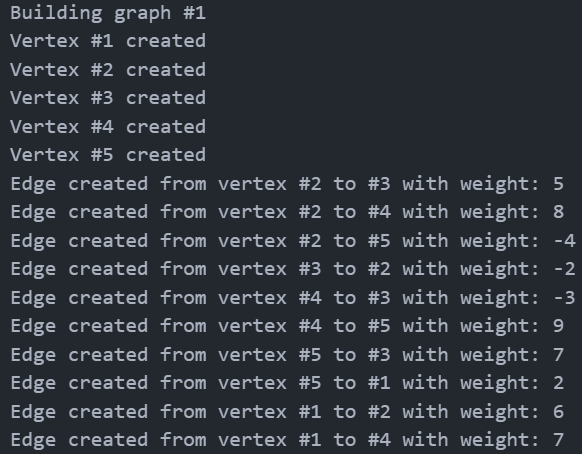
\includegraphics{images/Graph1_ParseBuild.png}
\end{center}

\subsection{Single Source Shortest Path Algorithm} \label{Graph_SSSP}

\section{Spices \& Knapsacks} \label{SpiceKnapsack}
TODO:
\begin{itemize}
   \item TODO:
\end{itemize}

\subsection{Parsing \& Building} \label{SpiceKnapsack_ParseBuild}
TODO:
\begin{center}
   \lstinputlisting[language=C++, caption=Parsing Implementation, firstline=1, lastline=5]{Parse.h}
\end{center}
TODO:
\begin{center}
   \lstinputlisting[language=C++, caption=Building Implementation, firstline=1, lastline=5]{Build.h}
\end{center}
TODO:
\begin{center}
   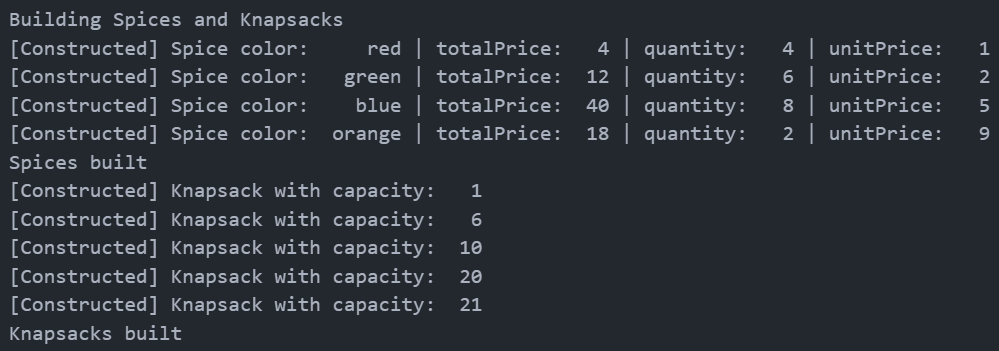
\includegraphics{images/SpiceKnapsack_ParseBuild.png}
\end{center}

\subsection{Fractional Knapsack Algorithm} \label{SpiceKnapsack_FKA}

\section{Clean Up} \label{CleanUp}
\begin{center}
   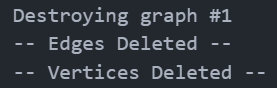
\includegraphics{images/Graph1_CleanUp.png}
\end{center}
TODO:
\begin{center}
   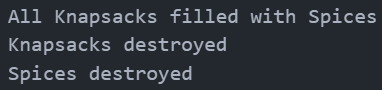
\includegraphics{images/SpiceKnapsack_CleanUp.png}
\end{center}
TODO:

\end{document}
